\chapter{Algoritmo \texttt{BFS}}

La prima cosa è guardare la struttura dei dati, esploriamo alcune
alternative e poi esaminiamo ciò che abbiamo allo stato dell'arte.
È fondamentale comprendere bene la struttura dei dati e l'algoritmo.
Affronteremo anche il problema del load balancing, che è particolarmente
rilevante in questo contesto.

\section{Rappresentazione del grafo in \texttt{GPU}}

Tra le varie rappresentazioni abbiamo:

\begin{itemize}
  \item Liste di adiacenza
  \item Matrice di adiacenza
  \item Edge list
\end{itemize}

\subsection{Matrice di Adiacenza}

La matrice di adiacenza è una rappresentazione comune dei grafi che memorizza
le relazioni tra i nodi in una matrice booleana. In una matrice di adiacenza,
ogni riga e colonna rappresenta un nodo del grafo, e il valore in posizione
\((i, j)\) indica se esiste un arco tra i nodi \(i\) e \(j\).

Nel caso di grafi pesati, si utilizza una matrice di adiacenza con valori
interi o in virgola mobile per rappresentare il peso degli archi:
\[
  M[i,j] = 
  \begin{cases} 
    0 & \text{se } i = j \\
    w(i,j) & \text{se } i \neq j \land (i,j) \in E \\
    \infty & \text{altrimenti}
  \end{cases}
\]

Il problema di tale approccio è che la matrice di adiacenza occupa spazio
\(O(V^2)\), che può essere inefficiente per grafi di grandi dimensioni.
Inoltre, la matrice di adiacenza richiede \(O(V^2)\) operazioni per
inizializzare e accedere ai dati, rendendo l'algoritmo meno efficiente.

\subsection{Liste di Adiacenza}

Le liste di adiacenza sono un'altra rappresentazione comune dei grafi
che memorizza la struttura del grafo in una serie di liste di adiacenza
per ogni nodo. Ogni lista contiene i nodi adiacenti al nodo corrispondente. Abbiamo quindi due liste, una per i nodi e una per gli archi. Nell'array dei vertici vengono memorizzati gli offset, ovvero il numero dei figli di ogni nodo. Nell'array degli archi vengono memorizzati i nodi figli.

La dimensione di questa rappresentazione è \(O(V + E)\), che è più
efficiente della matrice di adiacenza per grafi sparsi. Si tratta di un problema lineare in memoria, che è molto più efficiente per grafi di grandi dimensioni. Il problema è che l'accesso ai dati è più lento rispetto alla matrice di adiacenza, poiché richiede \(O(E)\) operazioni per accedere ai dati.

\subsection{Edge List}

L'edge list è una rappresentazione dei grafi che memorizza ogni arco del
grafo come una tupla di nodi. Questa rappresentazione è compatta e
richiede \(O(2E)\) spazio, rendendola ideale per grafi di grandi dimensioni.


\subsection{Scelta della Rappresentazione}
Nella scelta della rappresentazione del grafo, è importante
considerare le caratteristiche del grafo e le operazioni
che devono essere eseguite. Nel caso del \texttt{BFS}, è necessario considerare:
\begin{itemize}
  \item Il memory footprint
  \item L'accesso ai dati
  \item Tempo richiesto per trovare i figli dato un vertice
\end{itemize}

Consideriamo le più importanti ovvero la coalescenza e 
il load balancing. La tabella seguente confronta le varie rappresentazioni
in termini di utilizzo dello spazio, efficienza dell'accesso, bilanciamento
del carico, e coalescenza:

\begin{table}[H]
  \centering
  \caption{Confronto delle rappresentazioni di grafi}
  \begin{tabular}{|c|c|c|c|c|c|}
    \hline
    Rappresentazione & Spazio & $(u,v)\in E$ & $(u,v) \in \text{adj}(v)$ &
    Load Bal. & Coalescenza \\
    \hline
    Matrice di Adiacenza & $O(V^2)$ & $O(1)$ & $O(V)$ & Sì & Sì \\
    Liste di Adiacenza & $O(V + E)$ & $O(\text{deg}(v))$ & $O(\text{deg}(v))$ & Difficile & Difficile \\
    Edge List & $O(2E)$ & $O(E)$ & $O(E)$ & Sì & Sì \\
    \hline
  \end{tabular}
\end{table}
\section{Algoritmo \texttt{BFS} sequenziale}

L'algoritmo \texttt{BFS} è un algoritmo di ricerca in ampiezza che esplora
tutti i nodi di un grafo a partire da un nodo sorgente. L'algoritmo visita
tutti i nodi adiacenti al nodo sorgente, poi i nodi adiacenti a questi nodi,
e così via, fino a quando non ha visitato tutti i nodi raggiungibili dal nodo
sorgente.

L'algoritmo \texttt{BFS} può essere implementato in modo sequenziale
utilizzando una coda per mantenere traccia dei nodi da visitare. L'algoritmo
visita i nodi in ordine di distanza dal nodo sorgente, garantendo che i
nodi più vicini vengano visitati prima dei nodi più lontani.

\begin{algorithm}[H]
\caption{BFS sequenziale}
\DontPrintSemicolon
\SetAlgoLined
\ForEach{vertex \(u \in V(G)\)}{
  \( u.\text{dist} = \infty \)\;
  \( u.\pi = -1 \)\;
}
\( v_0.\text{dist} = 0 \)\;
\( v_0.\pi = -1 \)\;
\( Q = \{v_0\} \)\;
\While{\(Q \neq \emptyset\)}{
  \( u = Q.\text{dequeue}() \)\;
  \ForEach{vertex \(v \in \text{adj}(u)\)}{
    \If{\(v.\text{dist} = \infty\)}{
      \( v.\text{dist} = u.\text{dist} + 1 \)\;
      \( v.\pi = u \)\;
      \( Q.\text{enqueue}(v) \)\;
    }
  }
}
\end{algorithm}

Nell'algoritmo \texttt{BFS} sequenziale, la coda \(Q\) viene utilizzata
per mantenere traccia dei nodi da visitare. L'algoritmo inizia impostando
la distanza di tutti i nodi dal nodo sorgente a \(\infty\), tranne il
nodo sorgente stesso, che ha distanza \(0\). Il nodo sorgente viene aggiunto
alla coda \(Q\), e l'algoritmo continua finché la coda non è vuota. Ad ogni
iterazione, il nodo \(u\) viene rimosso dalla coda e i suoi nodi adiacenti
vengono visitati. Se un nodo adiacente \(v\) ha distanza \(\infty\), la sua
distanza viene impostata a \(u.\text{dist} + 1\) e il nodo viene aggiunto
alla coda.


\section{Algoritmo \texttt{BFS} in \texttt{CUDA}}
Nella versione parallela, la coda verra utilizzata come 
frontiera.
L'idea è di utilizzare una frontiera per mantenere traccia
dei nodi da visitare, e utilizzare un kernel per visitare
i nodi adiacenti a ciascun nodo nella frontiera.

Il filtraggio serve a non considerare nodi la cui distanza non è infinito 
ed ad eliminare figli che hanno più padri.

\subsection{Possibili soluzioni}
Una possibile soluzione per rimuovere duplicati è l'utilizzo di una 
hash table, l'idea è quella che con delle chiamate a basso livello si 
riesca a prendere un nodo ed ad infilarlo nella hash table, se il nodo
deve essere controllato lo si controlla dalla hash table.

\subsection{Varie tecniche di implementazione}
\begin{itemize}
  \item Prefix sum esclusiva: è una tecnica che permette di calcolare
  la somma di tutti gli elementi precedenti ad un certo indice.
  Nella \texttt{BFS} serve quando ho una frontiera e devo allocare i nodi 
  alla varie thread. L'idea è di assegnare i nodi con un certo bilanciamento, 
  per capire se un nodo ha figli o meno.
  La prefix sum deve essere implementata in modo efficiente, in quanto
  è un'operazione critica per il bilanciamento del carico.
  \item Warp virtuali dinamiche:
  \item Parallelismo dinamico: permette che la ricorsione sia 
  implementata nel kernel, in modo che ogni thread possa chiamare
  la funzione ricorsiva. In questo modo le thread e i blocchi di 
  thread possono essere creati in modo dinamico e creati runtime.
  Il problema è che è pesantissimo.
  \item Ricerca degli archi.
  \item Single-Block vs Multi-Block: è possibile utilizzare un solo
  blocco di thread per eseguire l'intero algoritmo \texttt{BFS}, oppure
  utilizzare più blocchi di thread per eseguire l'algoritmo in parallelo.
  L'utilizzo di più blocchi di thread può migliorare le prestazioni
  dell'algoritmo, ma richiede una sincronizzazione tra i blocchi.
  \item Lettura/Scrittura coalescente.
\end{itemize}

\section{Appunti 27/06}

\subsection{Blocco singolo vs Multi blocco}
La calibrazione della threshold impatta nell'organizzazione della 
memoria condivisa di ogni stream multiprocessor.
la memoria condivisa si organizza in modi diversi rispetto 
al numero di blocchi.
Nella versione single block, la memoria condivisa è organizzata
con una grossa parte dedicata alla hash table e una parte dedicata 
alla frontiera attuale e alla prossima. Nel caso multi block
la frontiera è gestita nella memoria globale, ma la memoria condivisa
ha un numero di variabili e ogni blocco di thread ha la 
propria hash table.
\subsubsection{Single Block tempo}
\[
  \texttt{F\_threashold} = \texttt{max\_threads\_per\_block}
  \cdot K_5
\]
\[
\texttt{HashT}_{\texttt{size}} = 
\texttt{neaest\_power\_of\_2}(|\texttt{SM}| - \texttt{Var}_\texttt{size})
\]

\subsubsection{Multi Block tempo}
\[
  \texttt{HashT}_{\texttt{size}} =
  \texttt{nearest\_power\_of\_2}\left(
    \frac{(|\texttt{SM}| - \texttt{Var}_\texttt{size}) - K_6}{
      \texttt{max\_blocks\_per\_Multiprocessor}
    }\right)
\]

\subsection{Coalescenza di lettura/scrittura}
Se lasciamo lavorare le thread indipendentemente, si ha un problema
di totale non coalescenza. 
\begin{figure}[H]
  \centering
  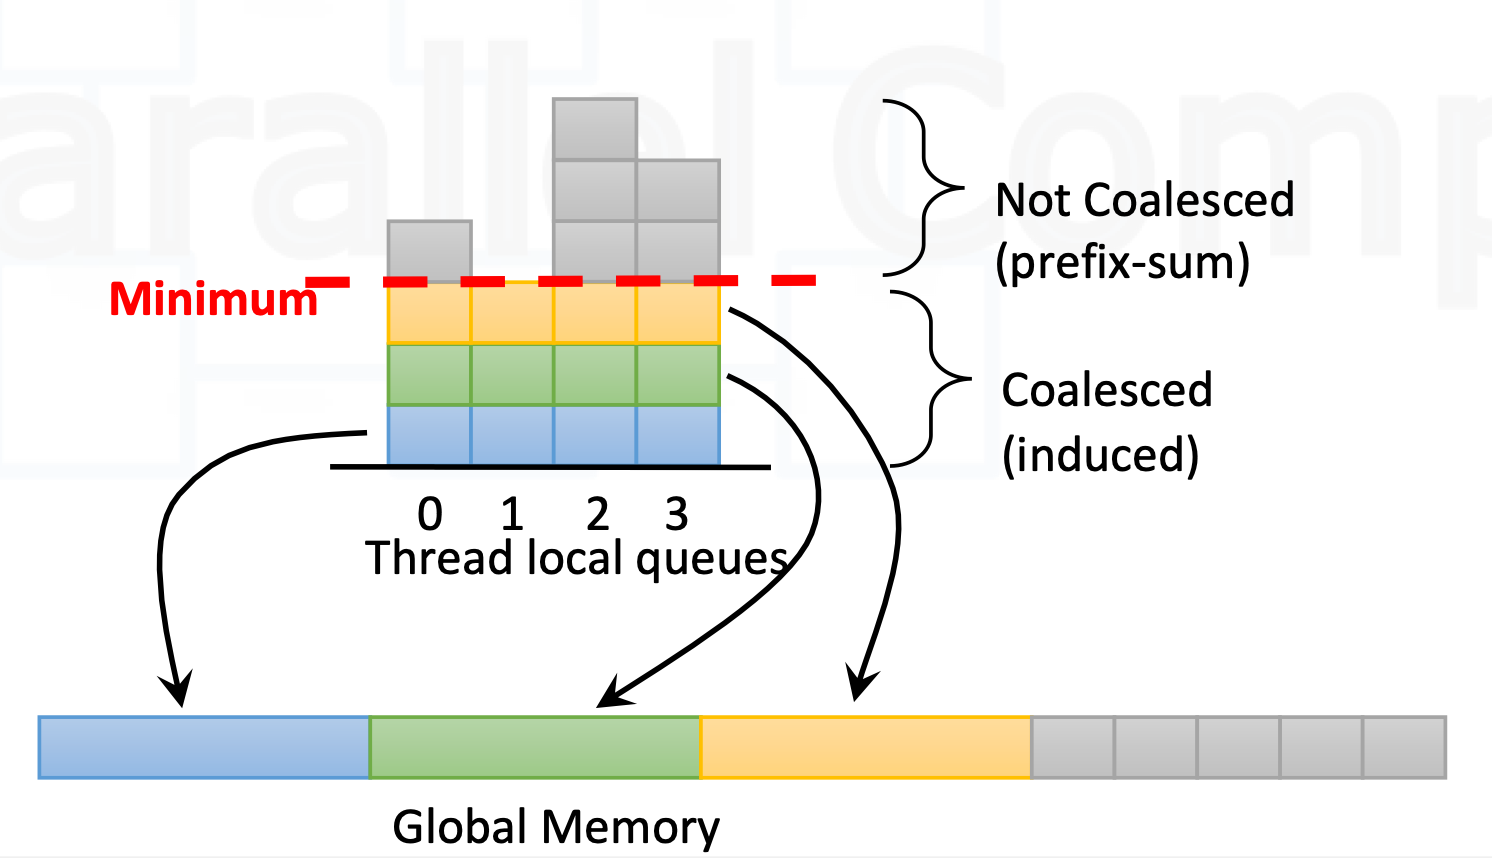
\includegraphics[width=0.8\textwidth]{img/coalescenza_bfs.png}
  \caption{Coalescenza di lettura/scrittura}
\end{figure}
\begin{figure}[H]
  \centering
  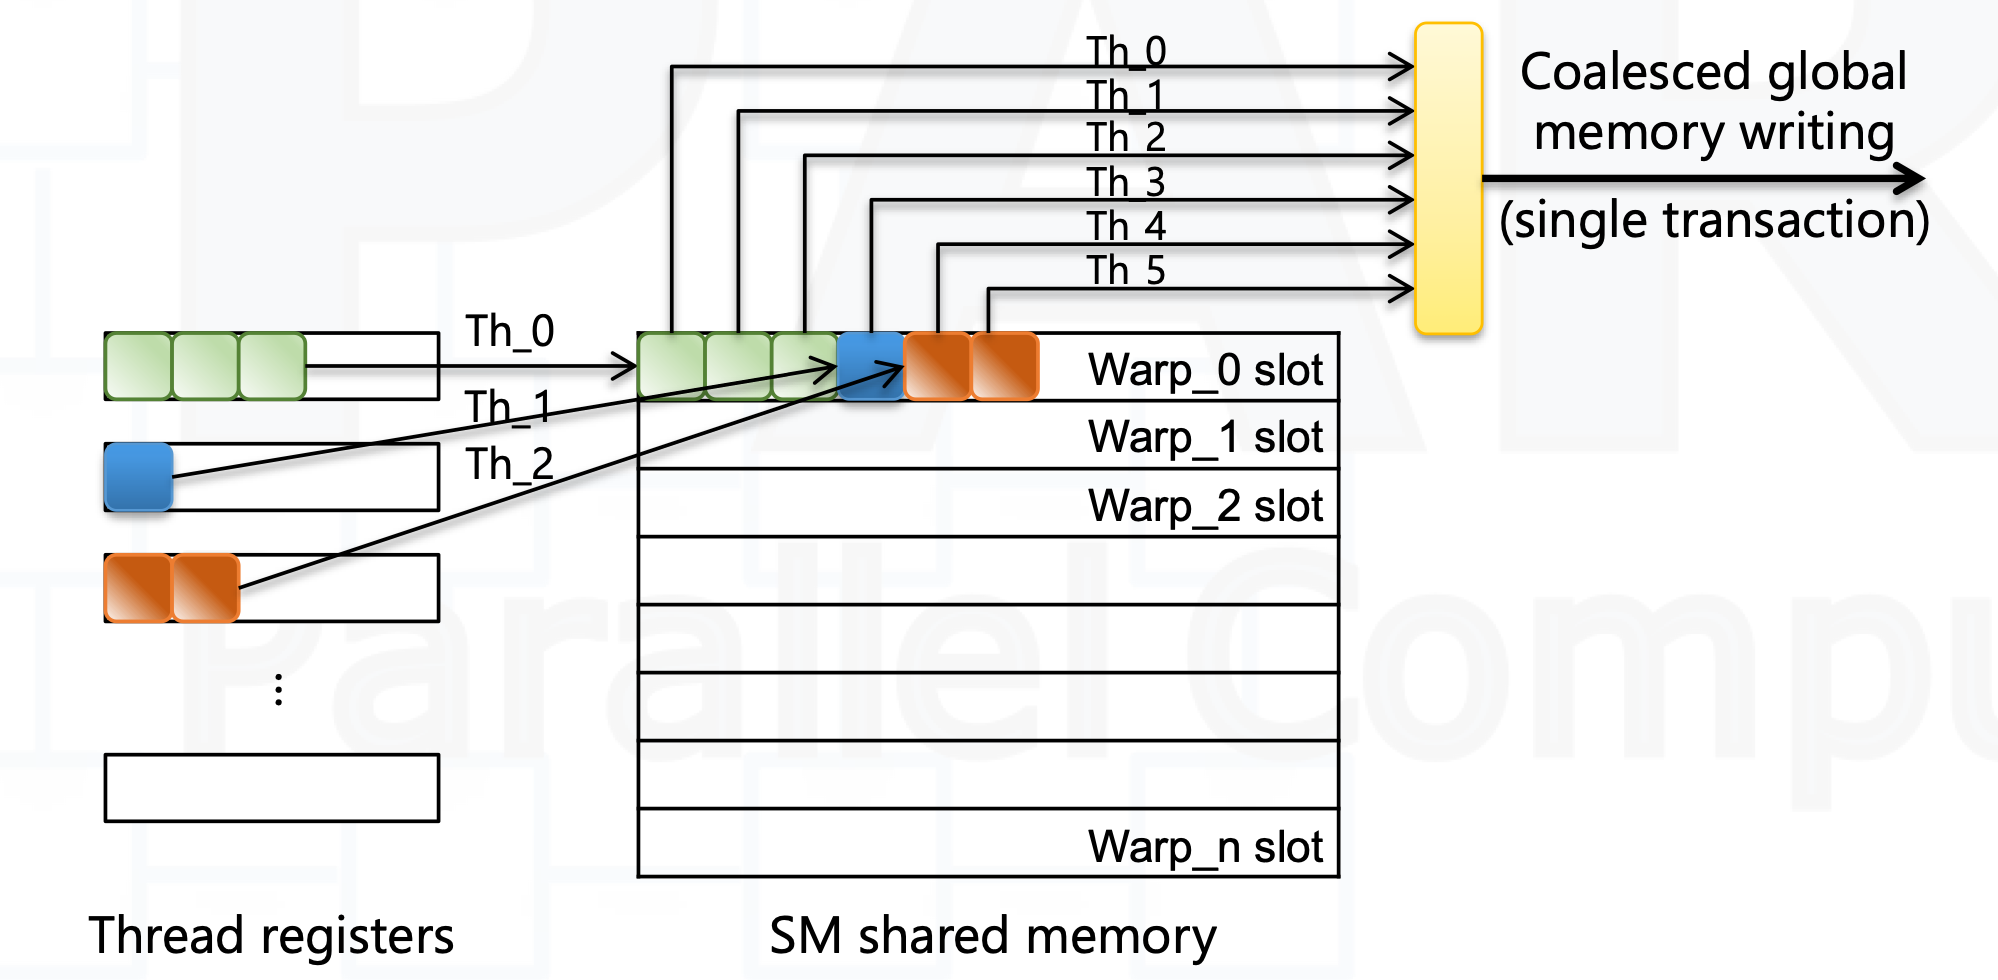
\includegraphics[width=0.8\textwidth]{img/coalescenza_bfs_2.png}
  \caption{Coalescenza di lettura/scrittura}
\end{figure}
